\documentclass[10pt]{article}

\usepackage[a4paper,margin=0.68in]{geometry}
\usepackage[T1]{fontenc}
\usepackage{lmodern}
\usepackage{microtype}
\usepackage{amsmath,amssymb}
\usepackage{booktabs,tabularx,array}
\usepackage{graphicx}
\usepackage[dvipsnames]{xcolor}
\usepackage{enumitem}
\usepackage{caption}
\usepackage{hyperref}

\hypersetup{colorlinks=true,linkcolor=NavyBlue,urlcolor=NavyBlue}
\setlength{\parindent}{0pt}
\setlength{\parskip}{4pt}
\setlist[itemize]{leftmargin=1.35em,itemsep=1pt,topsep=2pt}
\setlist[enumerate]{leftmargin=1.45em,itemsep=1pt,topsep=2pt}
\captionsetup{font=small,labelfont=bf,skip=4pt}
\renewcommand{\arraystretch}{1.12}

\definecolor{bdpblue}{HTML}{2C62A3}
\definecolor{softblue}{HTML}{EAF1F8}
\definecolor{softgray}{HTML}{F2F3F5}
\definecolor{darkgray}{HTML}{444444}

\newcommand{\keybox}[1]{%
  \begin{center}
  \colorbox{softblue}{\parbox{0.94\linewidth}{\small #1}}
  \end{center}}
\newcommand{\good}[1]{\textcolor{ForestGreen}{\textbf{#1}}}

\title{\vspace{-1.4em}\textbf{Calibrated Agentic-Serving Simulation and Minimal BDP}\\
\large A ten-minute technical note}
\author{}
\date{Frozen evidence: 20 paired held-out seeds, 80 programs arriving at $t=0$}

\begin{document}
\maketitle
\vspace{-1.8em}

\keybox{\textbf{Bottom line.} The simulator matches all nine declared public workload and service checks, while direct trace residuals are at most about 4.2\%. The current BDP policy is only a Bayesian remaining-work estimate plus one KV dual price. On held-out simulation, BDP reduces mean program completion time by 18.87\% versus FCFS and by 9.58\% versus Thunder. Giving the same index all future prompt/decode information exposes another 8.59\% mean-CT headroom, but does not improve the tail.}

\section{What is calibrated?}

The target is the public Qwen3-Coder-30B/vLLM-0.12, 80-program SWE-bench-style experiment from the GitHub results repository. Calibration is policy-independent: workload distributions, long-context service, KV allocation, prefix reuse, and recomputation are fixed before comparing scheduling policies.

\subsection*{Declared range checks: 9/9 pass}

\begin{table}[h]
\centering
\small
\begin{tabularx}{\linewidth}{>{\raggedright\arraybackslash}X r r c}
\toprule
Check & Simulator & Public range & Result \\
\midrule
Rounds per program & 15.18 & 14.6--15.3 & \good{pass} \\
Total decode tokens per program & 5929.6 & 5499.2--6629.6 & \good{pass} \\
CV of program decode tokens & 0.943 & 0.90--0.97 & \good{pass} \\
Submitted prompt tokens per program & 235905 & 235136--251274 & \good{pass} \\
Tool time per program (s) & 13.22 & 10.8--18.3 & \good{pass} \\
Prefill latency at 10k (ms/token) & 0.1297 & 0.11--0.13 & \good{pass} \\
Prefill latency at 40k (ms/token) & 0.1596 & 0.15--0.17 & \good{pass} \\
Decode latency growth at 40k & 7.0\% & 6--8\% & \good{pass} \\
Prefix drop/reuse cost ratio & 11.23 & 10--13 & \good{pass} \\
\bottomrule
\end{tabularx}
\end{table}

The earlier paired trace checks also measure shape, not only averages:

\begin{center}
\small
\begin{tabular}{l r@{\qquad}l r}
\toprule
Trace metric & Residual & Trace metric & Residual \\
\midrule
Size-run mean latency & $+0.7\%$ & KV utilization & $1.9$--$2.1\%$ \\
Running-sequence count & $0.2$--$4.2\%$ & Hazard-run cache hit & $-1.0\%$ \\
\bottomrule
\end{tabular}
\end{center}

Thus the worst reported direct residual is about 4.2\%; the central latency, KV, and cache residuals are roughly 1--2\%. This is sufficient for relative policy experiments under the calibrated setting. It is not a claim that the simulator predicts a different model, engine version, or arrival process without revalidation.

\clearpage
\section{Minimal BDP: one estimate and one price}

At each control step, BDP considers every ready program $i$. Let

\begin{equation}
\mu_i = \mathbb{E}[\text{remaining service work}_i\mid\mathcal H_i],
\qquad
q_i = \mathbb{E}[\text{KV footprint}_i\mid\mathcal H_i].
\end{equation}

The completion value and its KV density are

\begin{equation}
v_i=\frac{1}{\mu_i},
\qquad
d_i=\frac{v_i}{q_i}.
\end{equation}

The single dual price $\lambda$ is the marginal density $d_i$ at which the fractional candidate set fills the currently free KV capacity. BDP then uses one score:

\begin{equation}
\boxed{m_i=v_i-\lambda q_i.}
\end{equation}

Programs with $m_i>0$ are admitted in descending $m_i$, subject to actual KV and batch feasibility. This is Bayesian SERPT when KV is free ($\lambda=0$), and becomes more selective when KV is scarce. There is no learned value function, exact knapsack, cache reward, scenario branch, or tuned action threshold.

\subsection*{The Bayesian part}

The history $\mathcal H_i$ contains completed turns, current context, and stage. Remaining turns use a survival posterior. Decode scale uses one shrinkage update. For observed decode $x_{ir}$,

\begin{align}
\rho_{ir} &= P(\text{large component}\mid x_{ir},\text{current scale}),\\
z_{ir} &= (1-\rho_{ir})\frac{x_{ir}}{\bar x_{\rm small}}
       + \rho_{ir}\frac{x_{ir}}{\bar x_{\rm large}},\\
s_i &= \frac{\kappa+\sum_r z_{ir}}{\kappa+n_i},
\qquad \kappa=\frac{1}{\mathrm{CV}_{\rm program}^{2}}.
\end{align}

The predicted future decode is the calibrated mean times $s_i$. The observed context also caps predicted future turns using the workload's 35k next-input guard:

\begin{equation}
R_i=\min\!\left(R_i^{\rm survival},
\max\!\left(0,\frac{35000-c_i+\widehat x_i}{\bar p+\widehat x_i}\right)\right).
\end{equation}

These quantities produce $\mu_i$ and $q_i$; they do not add policy knobs.

\subsection*{What changed from the earlier BDP}

\begin{table}[h]
\centering
\small
\begin{tabularx}{\linewidth}{>{\bfseries}p{0.21\linewidth} X X}
\toprule
Part & Earlier version & Current minimal version \\
\midrule
Decode evidence & Raw token sum made one rare large turn look like persistent program heaviness. & Mixture responsibility separates a per-turn outlier from persistent scale. \\
Turn estimate & Survival posterior conditioned mainly on stage. & Same posterior, capped by the observable 35k context guard. \\
Action & Margin divided by admission blocks, with extra tie/fallback rules. & Direct margin $v_i-\lambda q_i$; PID only breaks exact ties. \\
Cache/packing & Router cache value and more packing logic were explored. & Removed; prefix reuse stays in the shared engine APC mechanism. \\
\bottomrule
\end{tabularx}
\end{table}

Held-out evidence supports the estimator changes: mixture-aware inference improves mean CT by 0.92\% over the old token-sum posterior (95\% CI 0.18--1.65\%), and context conditioning adds 1.44\%. Block normalization and the extra tie rules changed no simulated outcome on 40 seeds, so they were deleted.

\clearpage
\section{Held-out policy result}

All policies receive the same realized workloads on 20 seeds (20262101--20262120). Each run has 80 programs released together at $t=0$. FCFS and Thunder are the only baselines; BDP is the candidate.

\begin{table}[h]
\centering
\small
\begin{tabular}{lrrrrrr}
\toprule
Policy & Mean CT & P90 & P95 & Makespan & vs FCFS & vs Thunder \\
& (s) & (s) & (s) & (s) & mean CT & mean CT \\
\midrule
FCFS & 517.23 & 765.91 & 819.25 & 925.68 & -- & -- \\
Thunder & 464.51 & 719.41 & 774.38 & 892.11 & $+10.21\%$ & -- \\
\textbf{BDP} & \textbf{418.96} & \textbf{706.37} & \textbf{769.02} & 894.98 & \textbf{$+18.87\%$} & \textbf{$+9.58\%$} \\
\bottomrule
\end{tabular}
\caption{Average outcomes. A positive comparison means lower mean completion time.}
\end{table}

BDP beats FCFS on mean CT in 20/20 seeds; its paired improvement is 18.87\% (95\% CI 17.42--20.34\%). It beats Thunder on mean CT in 20/20 seeds by 9.58\% (95\% CI 8.00--11.25\%). Against Thunder, BDP also improves P90 by 1.79\%, while the P95 change is only 0.57\% and not significant. Thunder's mean makespan is 0.43\% lower than BDP's on paired runs, so the result is a strong mean-CT gain, not uniform dominance of every metric.

\begin{figure}[h]
\centering
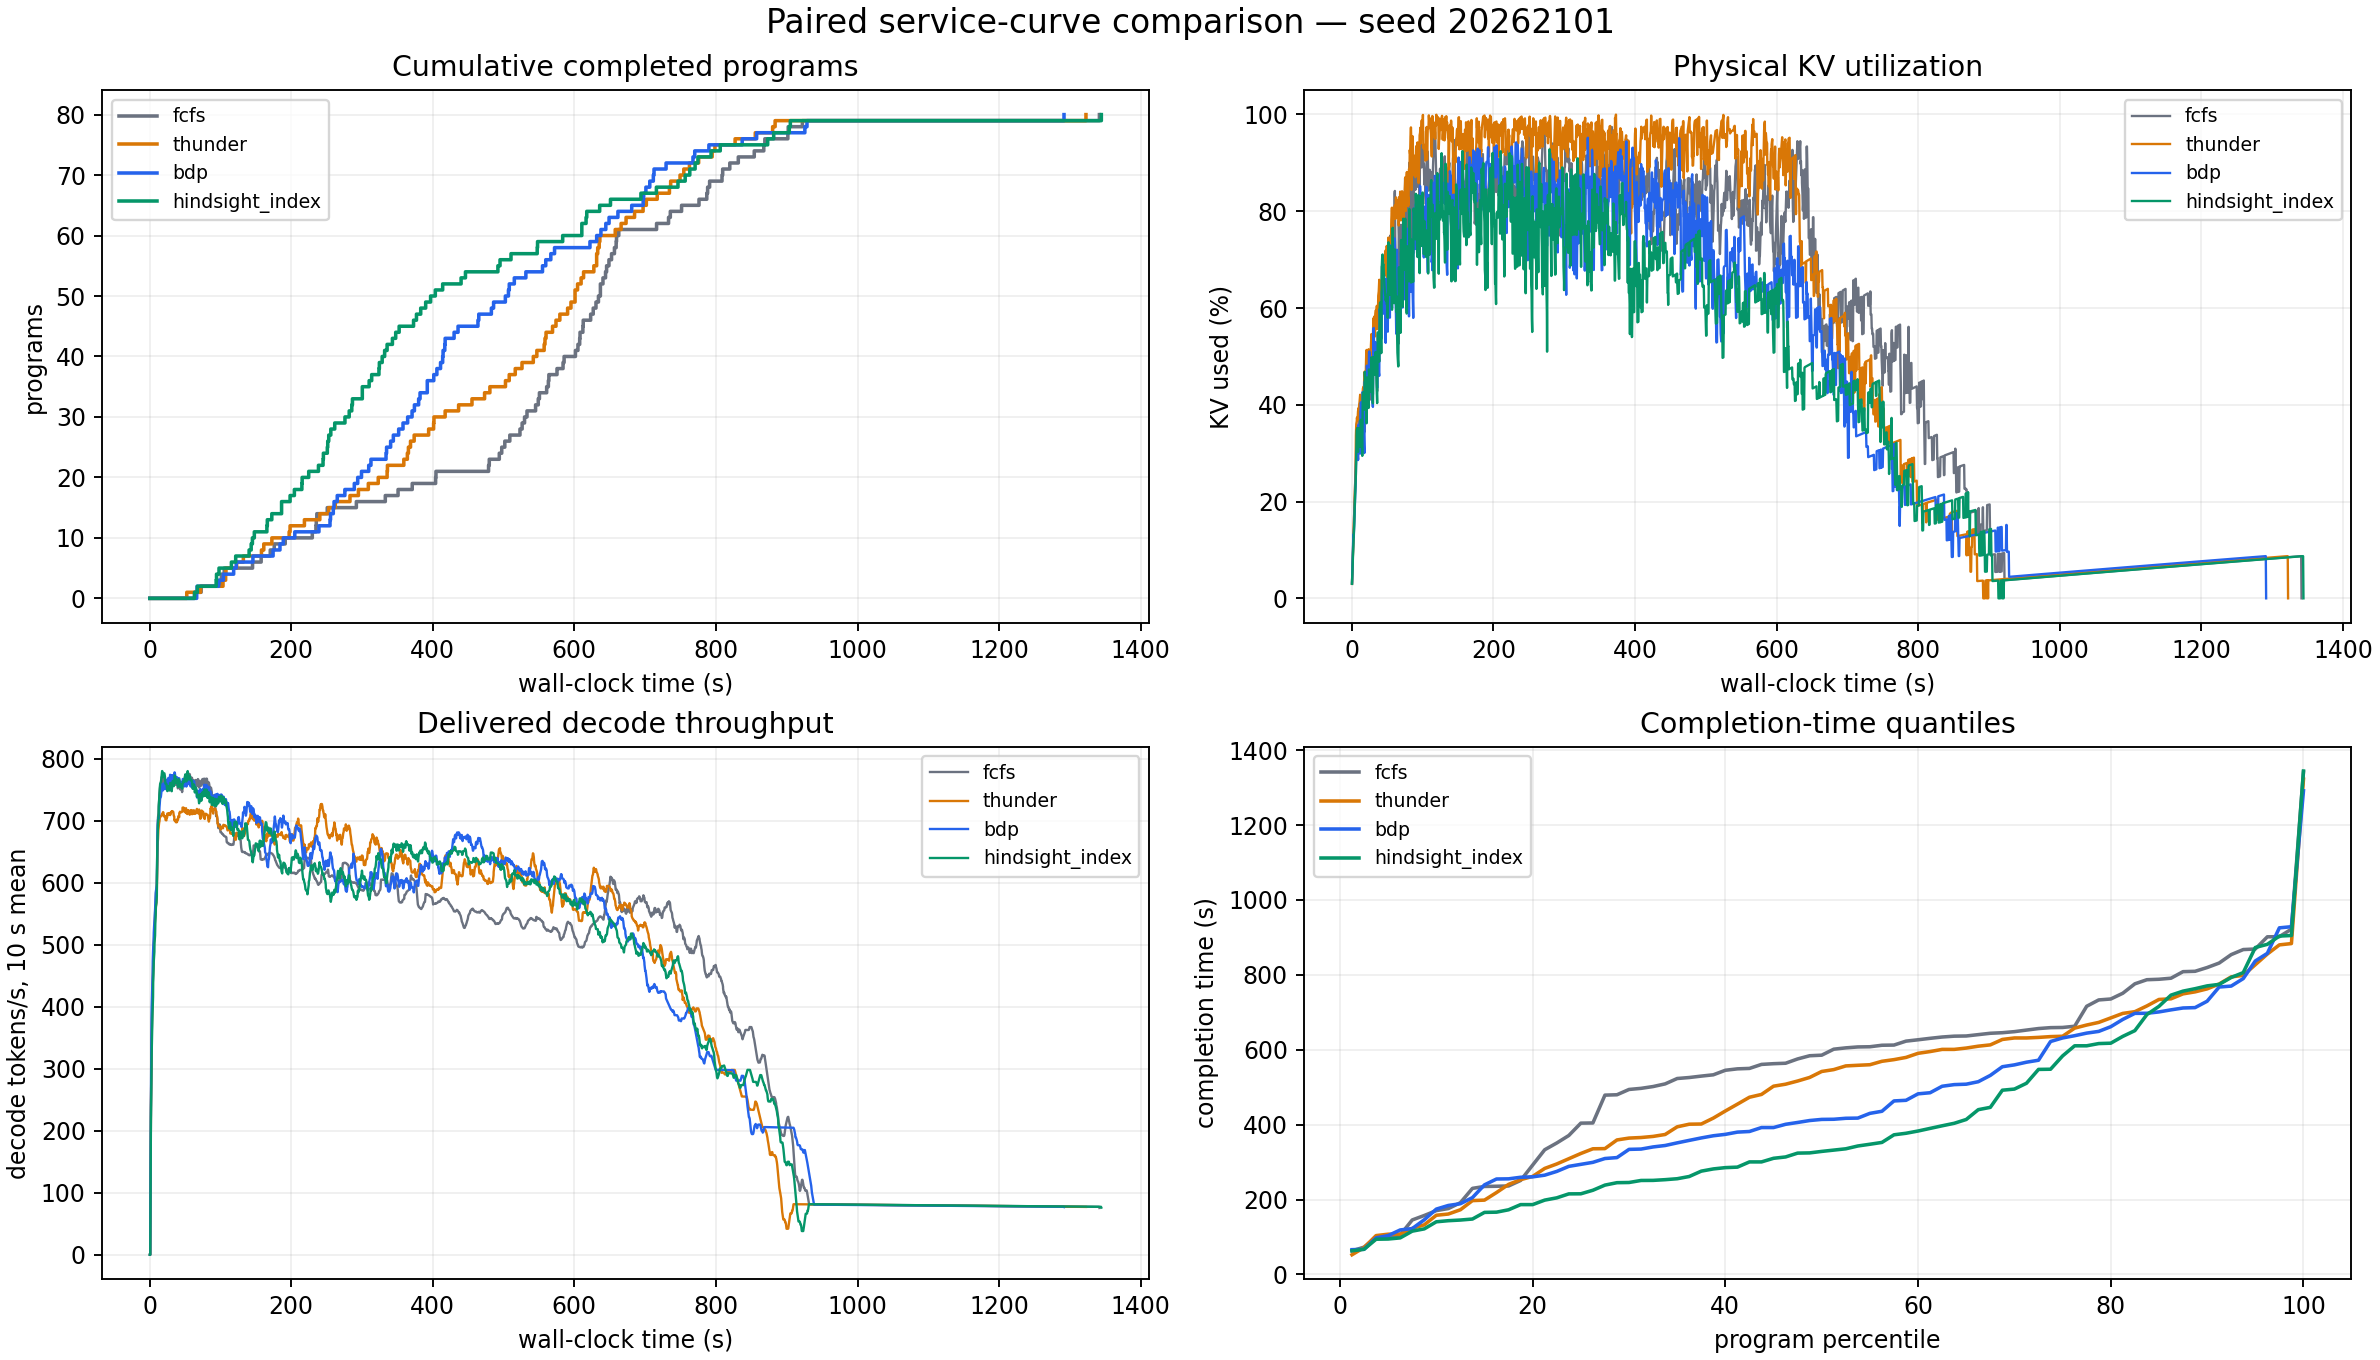
\includegraphics[width=0.98\linewidth]{../../results/service_curve/policy_comparison.png}
\caption{\textbf{Policy-level load curves} for paired seed 20262101. The panels show the completion ramp, physical KV load, decode throughput, and completion-time quantiles. BDP moves the completion curve left mainly during the congested early/middle window while keeping the tail close to Thunder.}
\end{figure}

\clearpage
\section{Where the load-curve gain comes from}

The aggregate curve can hide which programs are being served. The program-state timeline below expands the same BDP run into READY/PREFILL/DECODE/TOOL states. It shows repeated admission choices over the overloaded window, rather than a one-time ordering decision at $t=0$.

\begin{figure}[h]
\centering
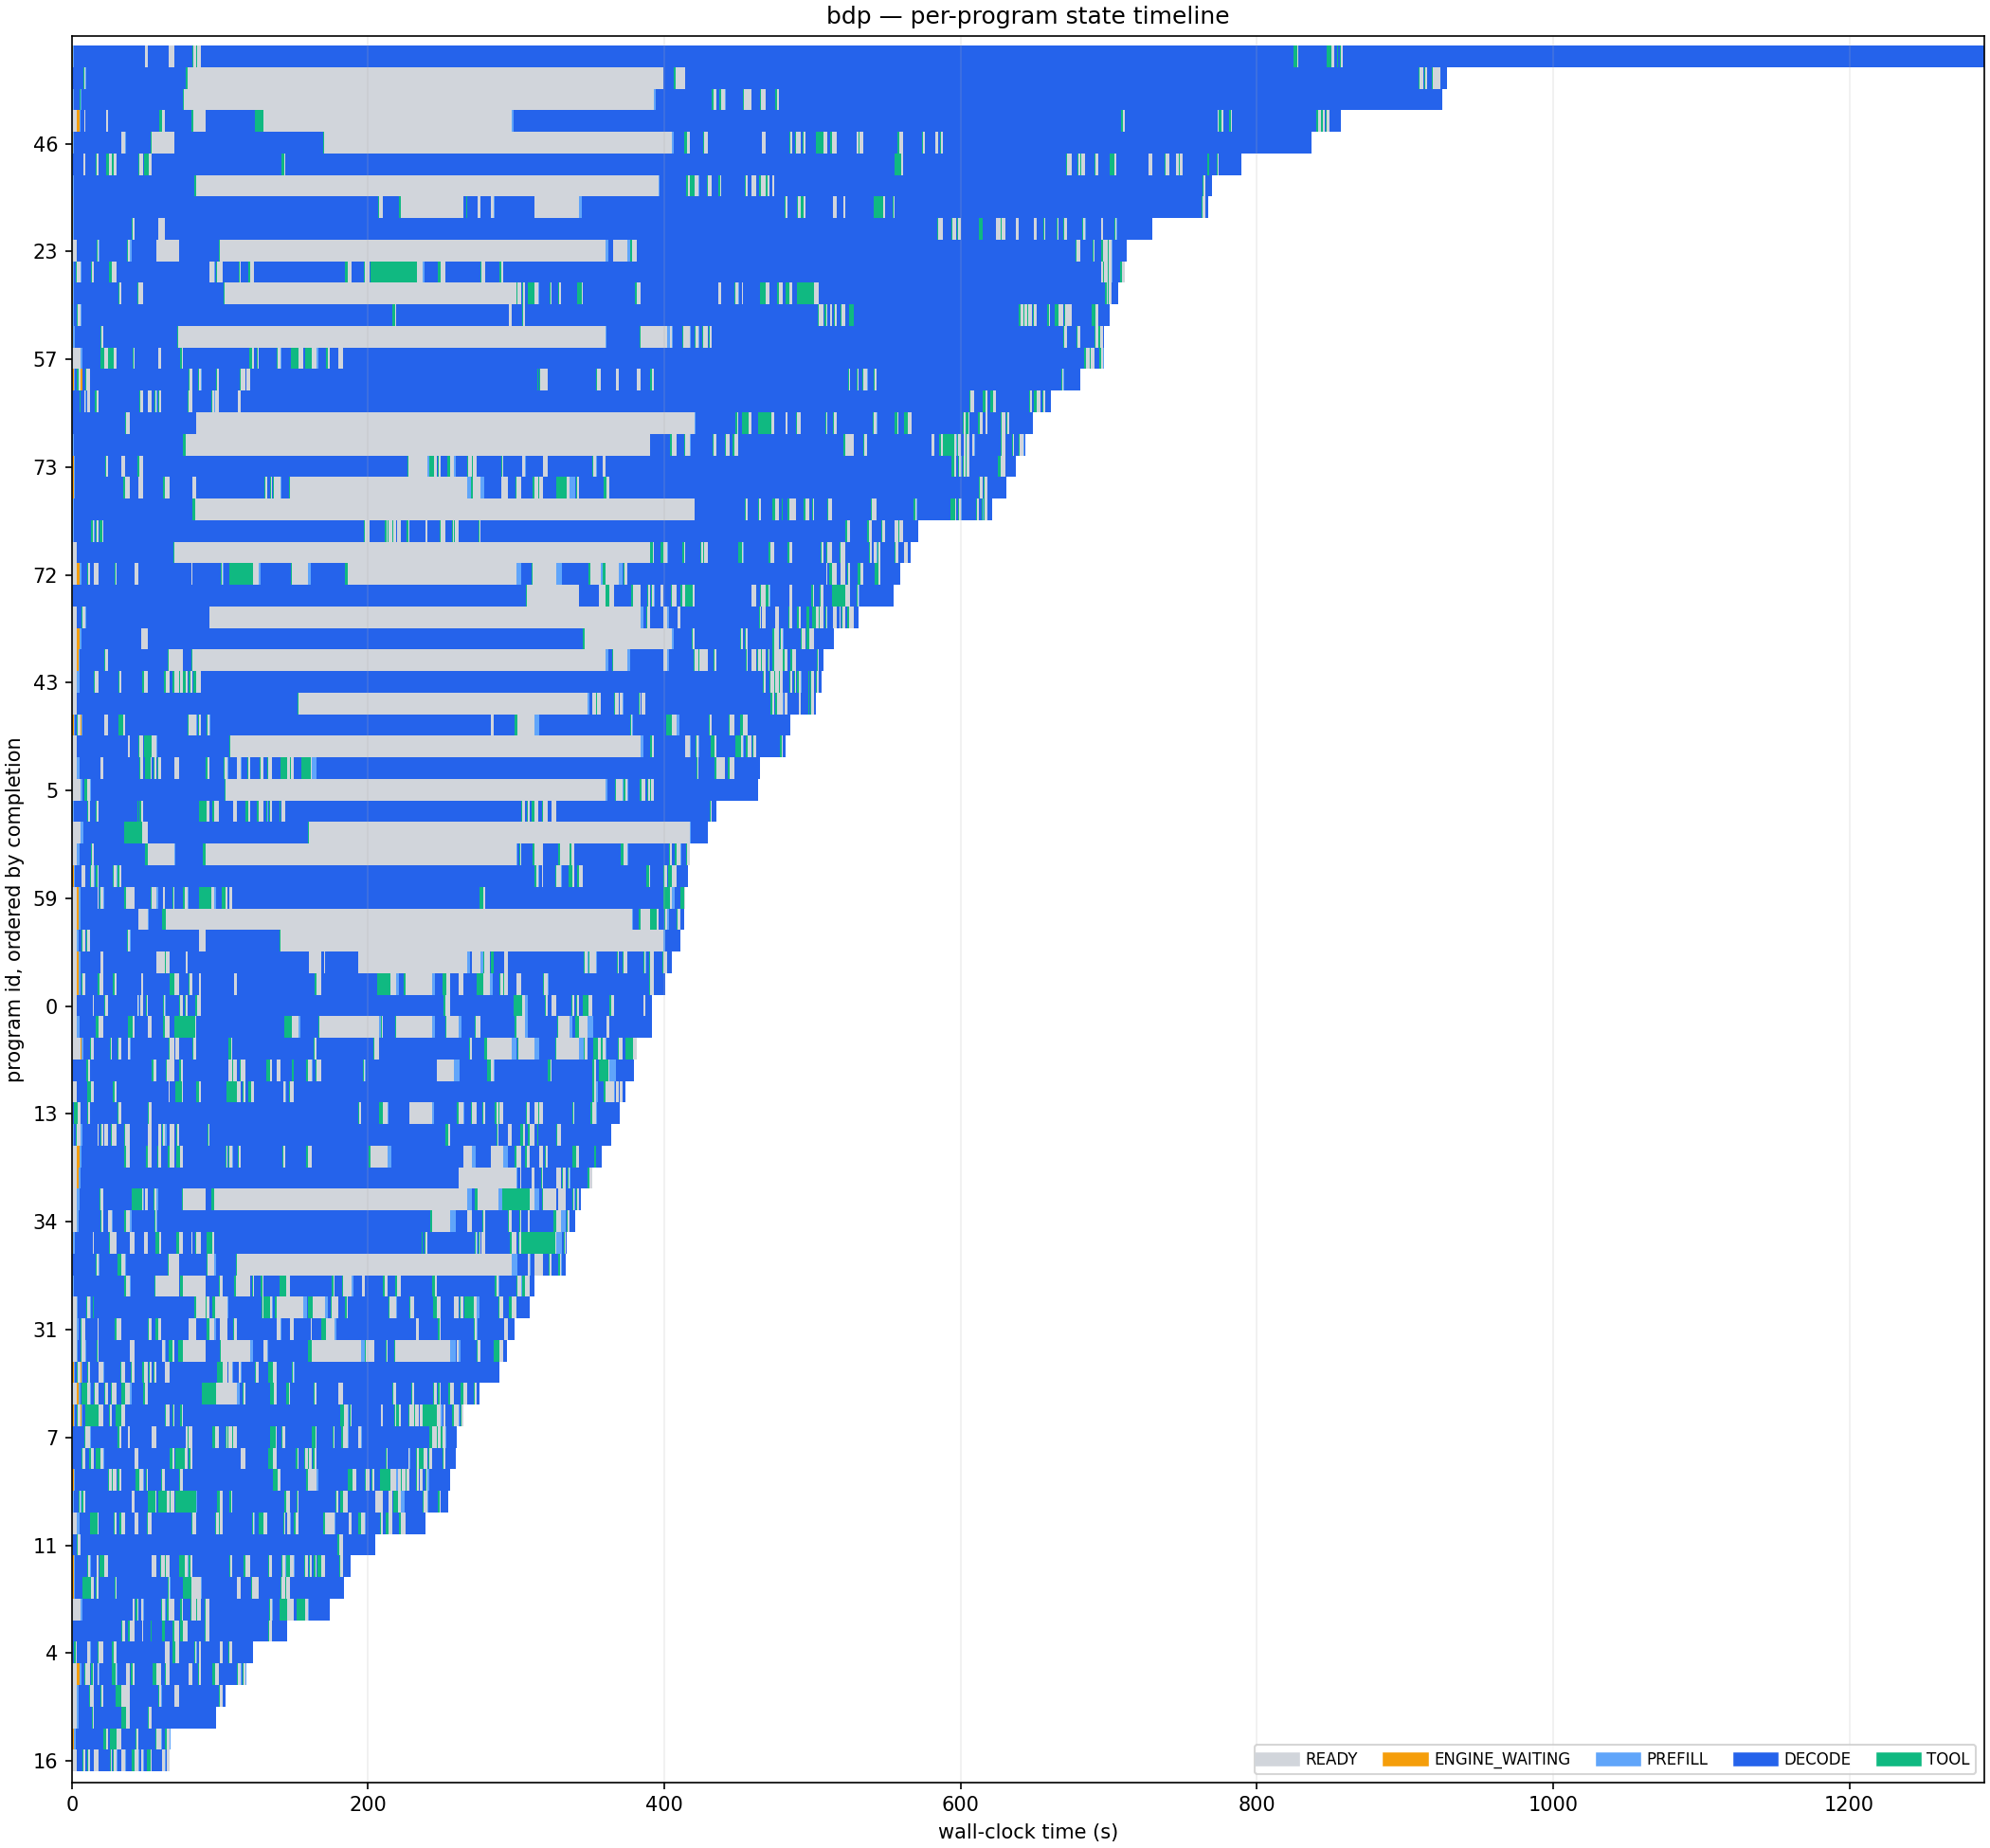
\includegraphics[width=0.94\linewidth,height=0.72\textheight,keepaspectratio]{../../results/service_curve/program_timeline_bdp.png}
\caption{\textbf{Program-state load timeline} for BDP, seed 20262101. Each row is one program; color changes expose service bursts, tool pauses, and the programs deliberately deferred under KV pressure.}
\end{figure}

The two figures answer different questions. The policy-level curve shows whether completions move earlier without a large tail penalty. The state timeline shows how the action sequence creates that curve. The remaining mismatch with hindsight is concentrated in repeated early/middle decisions: causal BDP sometimes defers a program after an observed large decode even when that program's future decode is light.

\clearpage
\section{How much headroom remains with future decode information?}

The diagnostic oracles keep the same BDP action formula and replace exactly one uncertain input. They are not baselines and are not deployable policies.

\begin{table}[h]
\centering
\small
\begin{tabularx}{\linewidth}{>{\raggedright\arraybackslash}X r r r}
\toprule
Information supplied to the same index & Mean CT & Gain vs BDP & 95\% CI \\
\midrule
Causal context-aware BDP & 418.96 s & -- & -- \\
Exact remaining turn count & 417.02 s & $+0.50\%$ & $[-0.55,1.51]\%$ \\
Exact turns + latent decode scale & 405.96 s & $+3.15\%$ & $[2.12,4.22]\%$ \\
Exact turns + realized program-mean decode & 382.88 s & $+8.58\%$ & $[7.43,9.68]\%$ \\
Exact ordered future prompts and decodes & 382.82 s & $\mathbf{+8.59\%}$ & $[7.57,9.59]\%$ \\
\bottomrule
\end{tabularx}
\end{table}

\keybox{\textbf{Interpretation.} Knowing the exact remaining turn count alone offers almost nothing. The dominant missing signal is each program's future average decode heaviness. Exact ordering of every future decode adds essentially nothing beyond that average under the current index. Therefore the useful headroom is about 8.6\% in mean CT, and it points to program-level decode uncertainty or a new causal action model, not more packing heuristics.}

The 8.59\% number is not a Pareto upper bound. The full-information index leaves P90 statistically unchanged ($-0.20\%$), but worsens P95 by 1.31\% and makespan by 1.47\% relative to causal BDP. A future policy should therefore seek the earlier completion ramp while preserving BDP's tail, rather than copy hindsight blindly.

\subsection*{Three takeaways}

\begin{enumerate}
\item \textbf{The simulator is ready for relative algorithm work in this setting:} all declared checks pass and the measured trace mismatch is within about 4.2\%.
\item \textbf{BDP is already logically minimal:} Bayesian remaining work, expected KV footprint, and one capacity-clearing dual price. The current form removes action-side decoration that had zero effect.
\item \textbf{The next structural target is clear:} close part of the 8.6\% mean-CT information gap without regressing P90/P95/makespan. Exact turn prediction is not the bottleneck, and additional final-score heuristics are not supported by the evidence.
\end{enumerate}

\vfill
{\footnotesize\color{darkgray}
Evidence: \path{results/coder_calibration}, \path{results/algorithm_experiment},
\path{results/bdp_gap_experiment}, and \path{results/service_curve}.\\
Public repository: \url{https://github.com/Echoscd/Agent-Inference}.}

\end{document}
